
\setcounter{chapter}{2}
\chapter{System Design and Architecture}
\minitoc %insert la minitoc
\graphicspath{{Chapitre3/figures/}}

%\DoPToC
%==============================================================================
\pagestyle{fancy}
\fancyhf{}
\fancyhead[R]{\bfseries\rightmark}
\fancyfoot[R]{\thepage}
\renewcommand{\headrulewidth}{0.5pt}
\renewcommand{\footrulewidth}{0pt}
\renewcommand{\chaptermark}[1]{\markboth{{\chaptername~\thechapter. #1 }}{}}
\renewcommand{\sectionmark}[1]{\markright{\thechapter.\thesection~ #1}}

\begin{spacing}{1.2}

%==============================================================================
\section*{Introduction}
This chapter presents the system design and architecture of the LLM-powered best practices enforcement system. Building on the business understanding and requirements established in Chapter~\ref{ch:business_understanding}, it details technical design decisions, architectural patterns, and system components that enable real-time, intelligent feedback for YouTube framework development.

The design follows traditional software engineering principles while incorporating modern AI technologies. This chapter covers the overall system architecture, component design, data models, and integration patterns that form the foundation of the implemented solution.

\section{System Architecture Overview}

\subsection{High-Level Architecture}
The system architecture is designed to integrate seamlessly into the developer's existing workflow while providing intelligent, context-aware feedback. It consists of two main components:

\begin{itemize}
    \item \textbf{IDE:} The developer's workspace, including the YouTube IDE Extension, which works with the currently open file and annotates results directly in the editor.
    \item \textbf{AI Agent Framework:} The processing layer containing the LLM Best Practices Agent, which performs code analysis and generates best practice suggestions.
\end{itemize}

\begin{figure}[H]
\centering
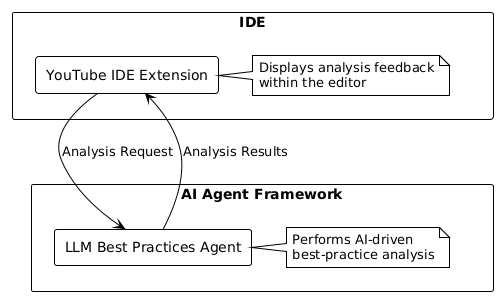
\includegraphics[scale=0.7]{images/high_level_system_architecture.png}
\caption{High-Level System Architecture}
\label{fig:system_architecture}
\end{figure}

Figure~\ref{fig:system_architecture} illustrates the separation between the IDE extension and the AI processing backend. The IDE provides immediate access to analysis capabilities, while the AI Agent Framework handles computationally intensive tasks. This separation allows independent scaling of AI capabilities without impacting IDE responsiveness.

\subsection{System Workflow}
The system operates through a streamlined workflow beginning when a developer triggers analysis via the IDE Extension (Figure~\ref{fig:sequence_diagram}).

\begin{figure}[H]
\centering
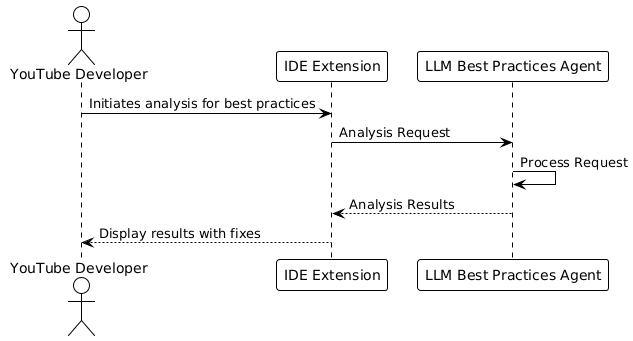
\includegraphics[scale=0.7]{images/sequence_diagram.png}
\caption{System Interaction Sequence Diagram}
\label{fig:sequence_diagram}
\end{figure}

The primary workflow includes:

\begin{enumerate}
    \item \textbf{Analysis Initiation:} The developer triggers analysis on the open file.
    \item \textbf{Request Submission:} The IDE Extension submits the request to the AI agent, identifying the target file.
    \item \textbf{Processing:} The agent performs best-practices analysis.
    \item \textbf{Result Delivery:} The agent returns structured findings.
    \item \textbf{Presentation:} The IDE Extension displays violations and suggested fixes in the editor.
\end{enumerate}

This workflow decouples the IDE from heavy computation, maintaining responsiveness while delegating analysis to the specialized agent framework.

\section{Components Design}

\subsection{LLM Best Practices Agent} 
The LLM Best Practices Agent is the core intelligence engine of the system. Its responsibilities include analyzing code, detecting violations of internal YouTube framework best practices, providing human-readable explanations, and suggesting actionable fixes. This component represents the intersection of AI capabilities with domain-specific software engineering expertise.

\subsubsection{Agent Architecture Options}
We explored multiple architectural paradigms for the agent, drawing inspiration from established AI agent patterns~\cite{microsoftAgentPatterns}. Figure~\ref{fig:agent_comparison} illustrates the fundamental differences in control flow between the two main options.

\begin{figure}[H] 
    \centering 
    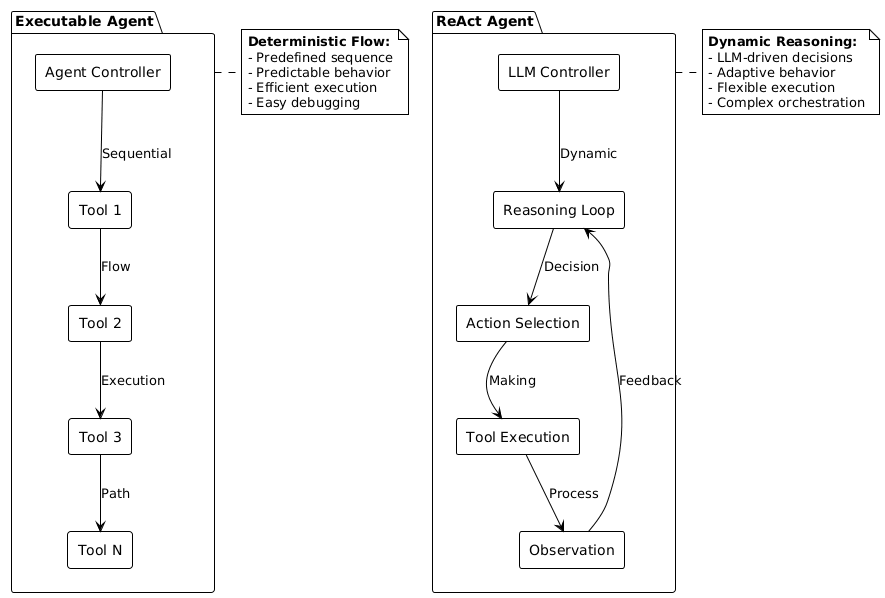
\includegraphics[scale=0.6]{images/agent_architecture_comparison.png} 
    \caption{Comparison of Executable Agent vs. ReAct Agent Architectures} 
    \label{fig:agent_comparison} 
\end{figure}

\begin{itemize}
    \item \textbf{ReAct Agent:} This architecture integrates \emph{reasoning and acting} loops. The LLM decides the next action, executes it, observes outcomes, and continues iterating. While highly flexible and capable of dynamic decision-making, ReAct agents introduce variability in execution flow, increased token consumption, and difficulty in guaranteeing deterministic outcomes.
    
    \item \textbf{Executable Agent:} The Executable Agent pattern~\cite{microsoftAgentPatterns} orchestrates a deterministic, predefined workflow. Control flow is explicitly encoded, with the LLM primarily responsible for domain-specific processing within each tool rather than orchestrating overall behavior. This approach provides predictable behavior, easier debugging, structured tool integration, and efficient token usage.
\end{itemize}

Each option has trade-offs:

\begin{itemize}
    \item \emph{ReAct}: High flexibility, adaptive reasoning, but non-deterministic and potentially higher latency/cost.
    \item \emph{Executable}: Predictable, maintainable, supports modular tool orchestration, but less flexible for emergent reasoning scenarios.
\end{itemize}

\subsubsection{Processing Strategy Options}
For handling multiple violations in a single file, we considered three strategies:

\begin{itemize}
    \item \textbf{Fully Sequential:} Processes violations one at a time, ensuring maximal reliability and deterministic outcomes. However, this introduces latency for large files with many violations.
    
    \item \textbf{Fully Parallel:} Processes all violations concurrently to maximize throughput. While performant, this increases complexity in managing concurrency, resource contention, and error handling.
    
    \item \textbf{Hybrid Approach:} Limits parallel execution to a controlled number of concurrent violations. This balances throughput and stability, leveraging parallelism without overloading resources or compromising reliability.
\end{itemize}

\subsubsection{Core Tools Architecture}
To maintain modularity and separation of concerns, the agent workflow is decomposed into specialized tools, each responsible for a specific step of the best practices enforcement pipeline:

\begin{itemize}
    \item \textbf{File Reading Tool:} Retrieves complete file content and metadata. Ensures full context for downstream analysis.
    
    \item \textbf{Code Analysis Tool:} Performs semantic and structural analysis, detecting violations against internal framework rules. Integrates static analysis heuristics with LLM-based reasoning.
    
    \item \textbf{Violation Explanation Tool:} Converts raw violations into human-readable explanations, providing actionable insight and contextual rationale for developers.
    
    \item \textbf{Code Fix Tool:} Suggests concrete corrective actions for each violation. Balances automated recommendations with developer flexibility, allowing acceptance, modification, or rejection.
    
    \item \textbf{Result Consolidation Tool:} Aggregates outputs from all tools into a structured response consumable by the IDE extension, ensuring clear and contextually accurate presentation.
\end{itemize}

\subsubsection{Integration with LLM Infrastructure}
The agent interfaces with an internal AI platform hosting multiple LLM models. Key design considerations include:

\begin{itemize}
    \item \textbf{Model-Agnostic Orchestration:} The architecture supports seamless adoption of new models without modifying the agent workflow.
    \item \textbf{Stable Interfaces:} Each tool interacts with the LLM via encapsulated, stable APIs to ensure maintainability.
    \item \textbf{Long-Term Flexibility:} New analysis rules or models can be integrated without architectural changes.
\end{itemize}

\subsection{Evaluation Framework for Architecture Decisions}
Given the complexity and multiple viable options for agent architecture and processing strategies, empirical evaluation is essential. Decisions cannot be based solely on intuition; performance, reliability, and quality need to be measured under realistic conditions.

\subsubsection{Test Suite Framework}
A set of 12 test cases was designed to cover a representative variety of scenarios, including:

\begin{itemize}
    \item Files with few versus many violations
    \item Simple versus complex violation patterns
    \item Edge cases where violations overlap or conflict
    \item Different programming constructs and language features
\end{itemize}

This diversity ensures that evaluations measure robustness across real-world conditions.

\subsubsection{LLM-as-a-Judge Methodology}
To assess output quality, we adopted an \emph{LLM-as-a-Judge} methodology. Instead of relying on brittle string matching, which can fail to recognize semantically correct outputs expressed differently, a separate LLM acts as an impartial evaluator:

\begin{itemize}
    \item Compares agent outputs against gold-standard solutions.
    \item Evaluates semantic correctness, completeness, and clarity.
    \item Scores explanations, suggested fixes, and overall alignment with framework best practices.
\end{itemize}

This approach enables robust evaluation of both ReAct and Executable workflows while capturing the nuances of human-readable explanations and context-aware fixes.

\subsubsection{Key Metrics}
The evaluation framework measures three primary dimensions:

\begin{itemize}
    \item \textbf{Accuracy:} Semantic correctness of analysis results and suggested fixes, as judged by the LLM evaluator.
    \item \textbf{Latency:} End-to-end response time, ensuring real-time usability in the IDE.
    \item \textbf{Cost:} Token consumption, API usage, and compute resource requirements.
\end{itemize}

\subsubsection{Candidate Architectures and Strategies}
The evaluation framework allows systematic comparison of all considered options:

\begin{itemize}
    \item \textbf{Sequential Executable Agent}
    \item \textbf{Parallel Executable Agent}
    \item \textbf{ReAct Agent}
\end{itemize}

Each candidate is assessed using the test suite and LLM-as-a-Judge methodology, producing data-driven insights into trade-offs between determinism, throughput, accuracy, and operational cost.
This combination of structured evaluation and modular design ensures that architecture and processing strategies can be selected with confidence, balancing performance, reliability, maintainability, and developer usability.


\subsection{YouTube IDE Extension}
The YouTube IDE Extension serves as the user-facing interface that seamlessly integrates the LLM Best Practices Agent into YouTube developers' daily workflow. Since YouTube developers are the primary target audience for this system, the YouTube IDE Extension was chosen as the natural entry point, leveraging their existing development environment and workflow patterns. This component is designed to provide intelligent, context-aware feedback while maintaining the responsiveness and familiarity that developers expect from their development environment. The feature becomes available when developers enable a user setting in the extension, and entry points only appear for files that belong to the internal YouTube framework for which we enforce best practices.

\subsubsection{Extension Architecture}
The YouTube IDE Extension serves as a lightweight client that orchestrates the interaction between developers and the AI analysis system. The architecture ensures responsiveness by delegating computationally intensive analysis to the specialized agent framework while handling user interface concerns, progress indication, and result presentation locally.

\subsubsection{User-Triggered vs. Automatic Analysis Design Decision}
A fundamental design decision for the IDE extension was whether to implement user-triggered analysis or automatic analysis. This choice significantly impacts user experience, system performance, and resource utilization.

The primary motivation for user-triggered analysis stems from the need to maintain developer productivity and system efficiency. LLM analysis is computationally expensive and resource-intensive, making continuous analysis impractical for maintaining IDE responsiveness. User-triggered analysis ensures that analysis occurs only when developers specifically request it, providing contextually relevant feedback at optimal moments without interrupting their workflow. This approach aligns with developer expectations of having control over their development environment while ensuring that computational resources are used efficiently.

Table~\ref{tab:analysis_approaches} summarizes the comparison of user-triggered vs. automatic analysis approaches:

\begin{table}[H]
\centering
\caption{Comparison of User-Triggered vs. Automatic Analysis Approaches}
\label{tab:analysis_approaches}
\begin{tabular}{|l|c|c|}
\hline
\textbf{Criteria} & \textbf{User-Triggered} & \textbf{Automatic} \\
\hline
User Control & $\checkmark$ & $\times$ \\
\hline
Resource Efficiency & $\checkmark$ & $\times$ \\
\hline
IDE Performance & $\checkmark$ & $\times$ \\
\hline
Contextual Timing & $\checkmark$ & $\times$ \\
\hline
Discoverability & $\times$ & $\checkmark$ \\
\hline
Always Current & $\times$ & $\checkmark$ \\
\hline
\end{tabular}
\end{table}

Based on this analysis, the user-triggered approach was selected as it provides superior resource management, user control, and system performance. The trade-offs in discoverability and stale state management are addressed through intuitive UI design and comprehensive feedback mechanisms.

\paragraph{Stale State Challenge}
The user-triggered approach introduces a fundamental design challenge: maintaining the relevance and accuracy of analysis results as developers continue modifying their code. This challenge requires balancing system responsiveness with result accuracy, ensuring that feedback remains useful throughout the development process.

\subsubsection{User Interface Design}
The YouTube IDE Extension is designed around two core interaction patterns: entry points for initiating analysis and feedback mechanisms for presenting results.

\paragraph{Entry Points}
The YouTube IDE Extension provides multiple entry points to ensure accessibility and discoverability for different user preferences and workflows:

\begin{itemize}
    \item \textbf{Visual Interface Integration}: Visual indicators are integrated into the development environment to provide immediate visibility of AI analysis availability, ensuring maximum discoverability while maintaining a clean interface.
    
    \item \textbf{Command-Based Access}: For developers who prefer keyboard-driven workflows, the extension provides command-based access through standard IDE navigation patterns, supporting both mouse-driven and keyboard-driven user interactions.
\end{itemize}

\paragraph{Feedback Mechanisms}
The YouTube IDE Extension employs three core feedback mechanisms designed to integrate seamlessly with existing development workflows:

\begin{itemize}
    \item \textbf{Progress Indication}: Real-time status updates during analysis processing to maintain developer awareness and system transparency.
    
    \item \textbf{Violation Display}: Presentation of analysis results using familiar interface patterns that leverage developers' existing knowledge of standard feedback mechanisms.
    
    \item \textbf{Contextual Suggestions}: Interactive code solutions that appear when developers interact with violation markers, providing actionable recommendations.
\end{itemize}


\subsubsection{User Interaction Flow}
The user interaction flow with the YouTube IDE Extension follows a structured pattern from analysis initiation to optional fix application:

\begin{figure}[H]
\centering
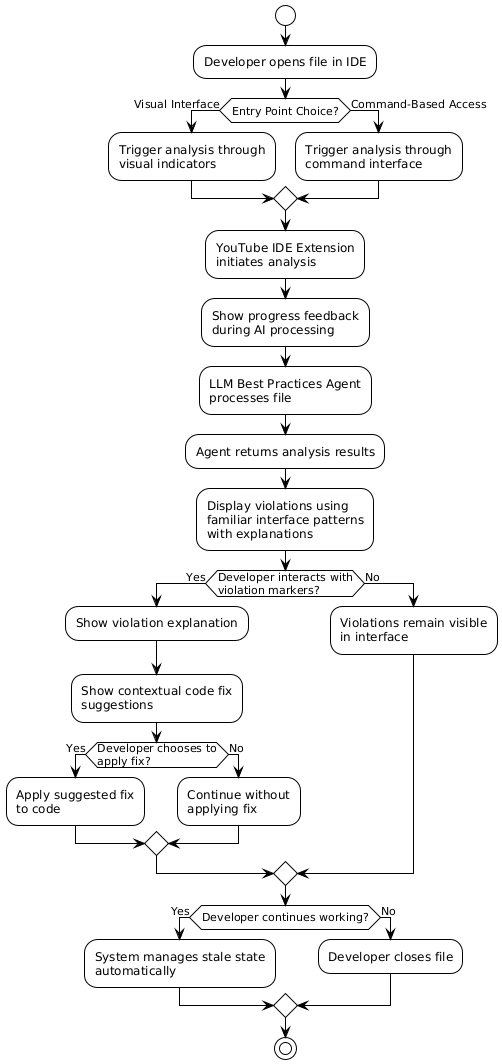
\includegraphics[scale=0.6]{images/user_flow.png}
\caption{YouTube IDE Extension User Interaction Flow: Complete developer journey from analysis trigger to fix application}
\label{fig:user_interface_flow}
\end{figure}

The flow demonstrates the core interaction pattern: developers initiate analysis through visual or command interfaces, receive progress feedback during processing, and interact with displayed violations to access explanations and optional fixes. This design ensures developers maintain control over their workflow while providing comprehensive feedback when requested.


\section{Data Models and Interfaces}

\subsection{Input/Output Specification}
The system's data models define the contracts between components, ensuring consistent communication and data exchange throughout the analysis pipeline. These interfaces establish clear boundaries between the IDE extension and the AI agent, enabling independent evolution of each component.

\paragraph{Analysis Request Format}
The YouTube IDE Extension sends analysis requests to the LLM Best Practices Agent using a minimal input format that identifies the target file for analysis. This design choice ensures that the agent can focus on its core responsibility of code analysis while maintaining security and proper workspace isolation. The request format includes the file path.

\paragraph{Analysis Response Format}
The agent returns a structured response containing the analysis results, error information, and optional metadata. The response format includes status information indicating success or failure, violation details with explanations and suggested fixes, and usage statistics for monitoring purposes. This standardized format ensures that the IDE extension can consistently process and display results regardless of the underlying analysis complexity.

\subsection{Convention Data Management}
The system's convention data model defines how YouTube framework best practices are structured, stored, and accessed throughout the analysis pipeline.

\paragraph{Convention Data Structure}
The convention data model captures best practice definitions as structured objects that support efficient programmatic access and analysis. Each convention definition includes essential metadata such as unique identifiers, descriptions, correct examples, and incorrect examples. This structure enables rapid lookup and context-specific retrieval during code analysis, with the design optimized for constant-time access patterns required by the agent's processing pipeline.

\paragraph{Storage Architecture Decision}
The system employs an in-memory storage approach using structured Python objects rather than external file-based or database storage. This design decision balances several architectural considerations:

\begin{itemize}
    \item \textbf{Data Characteristics}: Conventions are static during runtime, requiring no dynamic updates, making in-memory storage appropriate for performance-critical analysis.
    \item \textbf{Performance Requirements}: In-memory access ensures ultra-low-latency retrieval for real-time analysis, eliminating I/O overhead during agent execution.
    \item \textbf{Simplicity \& Reliability}: Structured Python objects provide type safety and eliminate parsing overhead while ensuring data integrity.
    \item \textbf{Resource Efficiency}: Conventions are loaded once at startup, minimizing runtime resource consumption and avoiding repeated file system access.
    \item \textbf{Architectural Flexibility}: The design allows future migration to external storage if multi-framework support or dynamic updates become necessary.
\end{itemize} 

\paragraph{Integration Interfaces}
The system defines minimal, versioned boundaries that keep components decoupled:

\begin{itemize}
    \item \textbf{IDE Extension Interface}: Contract between the YouTube IDE Extension and the LLM Best Practices Agent that defines the analysis request and response format, enabling independent evolution of UI and agent components.
    \item \textbf{Convention Access Interface}: Defines how the agent accesses convention definitions through in-memory lookup mechanisms, providing a stable boundary for data retrieval without external dependencies.
    \item \textbf{Monitoring Interface}: Captures usage statistics and performance metrics for system observability and evaluation purposes.
\end{itemize}


\subsection*{Conclusion}
The architecture of the LLM Best Practices Agent is defined by three central design decisions. First, the adoption of the Executable Agent paradigm ensures deterministic execution, structured tool orchestration, and predictable performance, avoiding the drawbacks of open-ended reasoning loops. Second, the hybrid parallel–sequential processing strategy balances efficiency with interpretability, allowing analyses to scale while maintaining transparency in intermediate results. Finally, the IDE extension provides a seamless developer experience, integrating feedback, explanations, and fixes directly into familiar workflows while managing state and staleness automatically. Together, these pillars create a robust, cost-efficient, and developer-friendly system for embedding AI-driven best practice enforcement into the coding environment.
%==============================================================================
\end{spacing}
